\section{重修微积分8——积分}

一元非负函数$ f(x) $从a到b的定积分,可以很直观地看成是这函数与x轴中[a,b]区间所夹的面积。在几何上,牛顿很直观地将[a,b]分割成细小的区间$ \Delta x $,以此为宽度的小长方块来填充或覆盖逼近这个面积,$ \sum_{i}f(x_i)\Delta x $,当Δx趋于零时它趋于这曲线所围的面积,莱布尼茨形象地把这个极限记为:$ \int_{a}^{b} f(x)dx $

。多元函数的多重积分是类推到高维体积的度量。

面积和高维体积按照这样计算的本质就是勒贝格测度。积分作为描述物理世界的数学模型,这是它所要求的属性。测度的计算是将整体切割成规范的部分,测算累加而成。上述牛顿的定义是按纵条切割的算法,叫做黎曼积分。面积也可以按横条来切割,把函数的值域区间细分,$ \sum _i  m(f^{-1}([y_i, y_i+\Delta y])) \Delta y $,算$ \Delta y $ 趋于零时的极限,这个算法收敛的极限叫勒贝格积分。(数学语言的定义见【1】,直观见图,图像来自网络下载)
\begin{figure}[h]
	\centering
	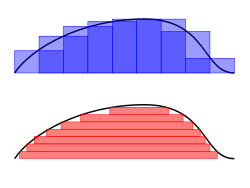
\includegraphics[width=0.7\linewidth]{pic/130332sliyik6hvp1iki1d.png}
	\caption{黎曼积分与勒贝格积分的直观区别}
	\label{fig:130332sliyik6hvp1iki1d}
\end{figure}

显然无论是用哪一种算法,它们计算所指的面积或体积是一样的,也应该相等的。将积分作为描述实践对象的数学模型,无论是用哪种测量计算方法,它们必须相等才有实用意义。这些面积或体积作为一种测度,如果按照不同的分割方法(即不同的积分定义)都有计算结果,在逻辑上也可证明是相等的。所以,如果黎曼积分和勒贝格积分都存在,它们相等。

如果函数具有负值,可以看成它是两个非负函数的相减。也就是两块面积体积或测度的相减,所以上述的结论也适用于一般的情况。

函数f在集合E上的勒贝格积分,记为$ \int_E f d m $,这里E是可测集,f是E上可测函数,m是E上的测度。当E是个区间时,它通常也用与黎曼积分相同形式的式子。请注意,对勒贝格积分,它只是沿用黎曼积分的形式记号,不再具有莱布尼茨那种对dx的符号解读。在可以缺省所指的测度和集合时,甚至将它记为$ \int_E f $或 $ \int f  $

因为所有黎曼可积的也是勒贝格可积,而且相等,借用相同积分形式的记法不会引起混淆。当你读论文里公式推导,看到不满足初等微积分相关的定理条件,居然也通行,不是作者不严谨,或误以为应用上不需要严谨,而是式子里指的是勒贝格积分。

勒贝格积分中测度、可测集,可测函数的术语吓住了许多对它们不熟悉的人,不敢使用。其实只要理解这是和黎曼积分一样应用,并具有更宽松应用条件的数学模型就不难了。黎曼积分的区域是可测集,能进行黎曼积分的函数是可测函数。黎曼积分都可写成勒贝格积分。在细节上:当E是一维时这里的勒贝格测度就是长度,二维时是面积,高维时是体积类推;说f是E上的可测函数,其定义是在E中f函数值大于任给一个数所有点形成的集合,都是可测集。大致说来,可测集包含了非数学专业人可以想象到的任何集合。迄今所知的勒贝格不可测集,都是用选择公理构造出来的无穷世界里的怪胎。如果你在物理或工程应用中涉及勒贝格积分,除非得到惊人违反常识的结果,大约都可放心地认为,你用到的都是可测集和可测函数。你大约还没有足够的运气和能力,构造出不可测集或不可测函数来犯错误。

既然这两种积分都一样,为什么黎曼积分用了几百年后,被称为经典分析而渐渐淡出,上个世纪初发展的勒贝格积分被广泛应用,并看作是近代分析的开端呢?

简单的答案是:应用黎曼积分在积分区域、积分函数及参与其他无穷过程时,有许多限制,而勒贝格积分解决了这些麻烦。它们是对相同应用的不同测算方法,就像原来用木尺丈量土地,现在改为用测距仪来测量一样,更有效的新方法必然会取代旧的,需要的只是熟悉。观念转换需要时间来消化,所读课本需要更新,个人则像是跟了不同师傅学了不同的功夫而已。

观念的不同带来了眼界的不同。经典分析一直徘徊在有限的视野和无穷的梦魇中。站在有穷世界的岸边,用无穷过程来窥视对岸的实无穷。想尽量保持有限世界的直观和逻辑上的严谨。这种囿于有限世界的观念和对无穷实质的回避,使得触及无穷时缩手缩脚,理论结果支离破碎。而勒贝格积分则基于包括有限和实无穷集合的测度研究上,以逻辑为骨架来拟合修正过去经验形成的概念。只要善于纠正陈旧观念形成的误区,在新的直观下,便能欣赏更广阔世界中简洁一致的美。

测度是从0到无穷大的量度。在包含着正负无穷大的扩充实数里,它们间的四则运算除了规定0乘无穷大仍为0外,其他都与中学关于无穷大的知识一致,包括了无穷大减无穷大没有定义。在勒贝格积分中,函数和积分的值域都是定义在这扩充的实数上。不难想象和证明,对于非负可测函数,勒贝格积分都存在。可测函数可以分解成两个非负可测函数之差,所以只要它俩的积分不都是无穷大,可测函数的积分都存在,在应用上都有意义。注意勒贝格积分存在,包括了它的积分值可能是无穷大的情况,所以勒贝格积分通常都存在。而勒贝格可积函数指的是积分值是有界的,显然,勒贝格可积等价于它是绝对可积的。

黎曼积分是定义在有界区间上有界函数的积分,这时勒贝格积分也有界,所以黎曼可积,勒贝格也是可积的。勒贝格积分定义在任何可测集上,包括可以黎曼积分的区间,和无界的全空间。黎曼积分要推广到无界的区间,它通常被定义为有界区间上积分的对称上下限无穷的扩展,在想象上比较直观,但这是个有疵瑕的形式扩展。例如,对于在0点从-1到1的阶跃函数,广义黎曼积分值是0,勒贝格积分不存在,对于周期函数也是如此。有些书上作为黎曼可积,勒贝格不可积的例子。但阶跃函数的广义黎曼积分,不满足平移不变性,若坐标向左或右平移一点,它的黎曼积分值就不同了。对周期函数如果黎曼积分的上下界不是对称地无穷扩展,它们的极限积分值也不一样。这用于描述物理世界,对应着测量的坐标变化和计算的方法不同,则意味着测算物理量的不同。所以对应于数学模型描述的对象,勒贝格不可积的结论正确地反映了这种不可计量的情况,广义黎曼积分则给出误导的答案。在推广到无穷的区域,广义的黎曼积分无论如何定义都有疵瑕。

黎曼积分最大的问题是,在与取极限、无穷级数、多重积分等运算的交换顺序,必须在很严格的条件下方为可行,这在应用上极不方便。实际上黎曼绝对可积的函数,在绝对值积分的范数下不是个完备的空间,这就像我们只在有理数域谈几何公式和代数应用,处处受到局限。从另一种观点来看,勒贝格积分可以定义为可积空间完备化的手段,它将函数绝对值黎曼积分为范数的计算方法更进,勒贝格可积函数是包含了黎曼可积函数的巴拿赫空间$ L^{1} $。【4】

为什么勒贝格积分会带来了这么多的便利?我们先用零测集牛刀小试。

黎曼积分在基本定义中假定被积的函数是连续的有界的,但应用中不一定都那么理想,可能有些间断点的“毛刺”,它的技术处理是分段来积分,然后将它们加起来,绕过这些疵点。在疵点是有限数目时,这样处理没有问题,但如果有无穷多个呢?

勒贝格积分告诉我们,如果这些疵点是零测集,把它们刨去换成任何数值,都不影响积分结果。黎曼积分和勒贝格积分如果同时存在,它们的数值必然相等。例如,Dirichlet函数D(x),当x是有理数时为1,无理数时为0;它在[0,1]区间的勒贝格积分为0,但不是黎曼可积的。我们知道可数个点集是零测集,有理数是可数的,所以是零测集,将这些点的函数值都置换成0,便是恒为0的常数值函数,这时黎曼积分也是0. 用这个方法“修理”黎曼积分中有疵瑕的函数,便得出黎曼积分的一个重要定理:

\kaishu\setlength{\leftskip}{1em}

区间[a,b]上函数f是黎曼可积的,必须且只需f在[a,b]上的不连续点是零测集。

\songti\setlength{\leftskip}{0em}


在积分和概率计算中都可以忽略零测集,这引入了常见的一个数学术语“几乎处处”(almost everywhere),简记为“a.e.”。如果两个函数不相等点的集合是零测集,叫做它们是“几乎处处相等”,它们的勒贝格积分相等。因此可以用一个几乎处处相等“良好的”函数来替代它计算。一个函数除了有个零测集外是有界的,叫做“几乎处处有界”。对积分的所有定理,可以把有界函数的条件换成“几乎处处有界”。闭区间上黎曼可积的函数,当且仅当是几乎处处连续的。

黎曼积分积分号里函数序列取极限,要在很强的条件下才能与积分号交换顺序。而“勒贝格控制收敛定理”说:在积分的集合上,只要它们的绝对值几乎处处不大于一个勒贝格可积函数,它们就几乎处处逐点收敛到一个函数,函数序列取极限就可以与勒贝格积分号交换顺序。

对于几乎处处一致有界的可测函数序列,勒贝格有界收敛定理给出更宽松的收敛要求,它只要这序列是按测度收敛就可以与积分号交换顺序了。什么是“按测度收敛”呢?就是说,这序列函数与其极限函数不同之处,将会趋于零测集。

对于$ \mathbb{R}^n $区间上勒贝格可积的函数,Fubini定理说,它的积分等于任何顺序的多重积分,也就是说可以任意地交换积分顺序。

牛顿—莱布尼茨公式描述了微分与积分的关系。记$ F'(x)=f(x) $,有 $ \int_a^b f(x)dx = F(b)-F(a) $ ,直观图像是,F曲线划分成n段折线,计算折线y轴上的增量与x轴增量之比,其导函数是当n趋近无穷大时,这些比值的极限。对这个导函数的积分,可以看成逼近导函数的这些折线比值与x轴增量的乘积累加的极限,很明显它是这些折线在y轴增量之和,因此等于这曲线在y轴数值之差。

在黎曼积分里这个定理要求被积函数在[a,b]上是连续的,或说原函数是连续可微的。在勒贝格积分里,我们有:原函数F在[a,b]上是绝对连续的,等价于它是勒贝格可积函数f的不定积分,且有牛顿—莱布尼茨公式关系。F几乎处处可导,其导数几乎处处等于f。这结论要比黎曼积分强多了,也更靠近直观想象。

仔细读过这篇文章,必要时将你应用积分推导的公式后面加个“(L)”,表明这是勒贝格积分,那么它“几乎处处”会让你免除许多严格条件限制的烦恼,和数学上不严谨的责难。

勒贝格积分除了与黎曼积分同样应用在$ \mathbb{R}^n $上,且有更自由积分区域外,还通用于任何定义有测度的抽象集合,例如随机过程在概率空间上的积分。勒贝格积分极大地提高了你的数学武功,只是你想深入其中纵横自如,则要走出历史旧观念的局限,改练无穷世界的测度基本功。


【扩展阅读】

\begin{enumerate}
	\item 维基百科,勒貝格積分
	\url{http://zh.wikipedia.org/wiki/\%E5\%8B\%92\%E8\%B2\%9D\%E6\%A0\%BC\%E7\%A9\%8D\%E5\%88\%86}
	
	\item 维基百科,维塔利集合\url{http://zh.wikipedia.org/wiki/\%E7\%BB\%B4\%E5\%A1\%94\%E5\%88\%A9\%E9\%9B\%86\%E5\%90\%88}
	
	\item 维基百科,微积分基本定理\url{http://zh.wikipedia.org/wiki/\%E5\%BE\%AE\%E7\%A7\%AF\%E5\%88\%86\%E5\%9F\%BA\%E6\%9C\%AC\%E5\%AE\%9A\%E7\%90\%86}
	
	\item 关肇直等,张恭庆,冯德兴,线性泛函分析入门,上海科学技术出版社,1979
\end{enumerate}

